\documentclass{standalone}
\usepackage{tikz}
\usetikzlibrary{patterns, positioning}

\begin{document}
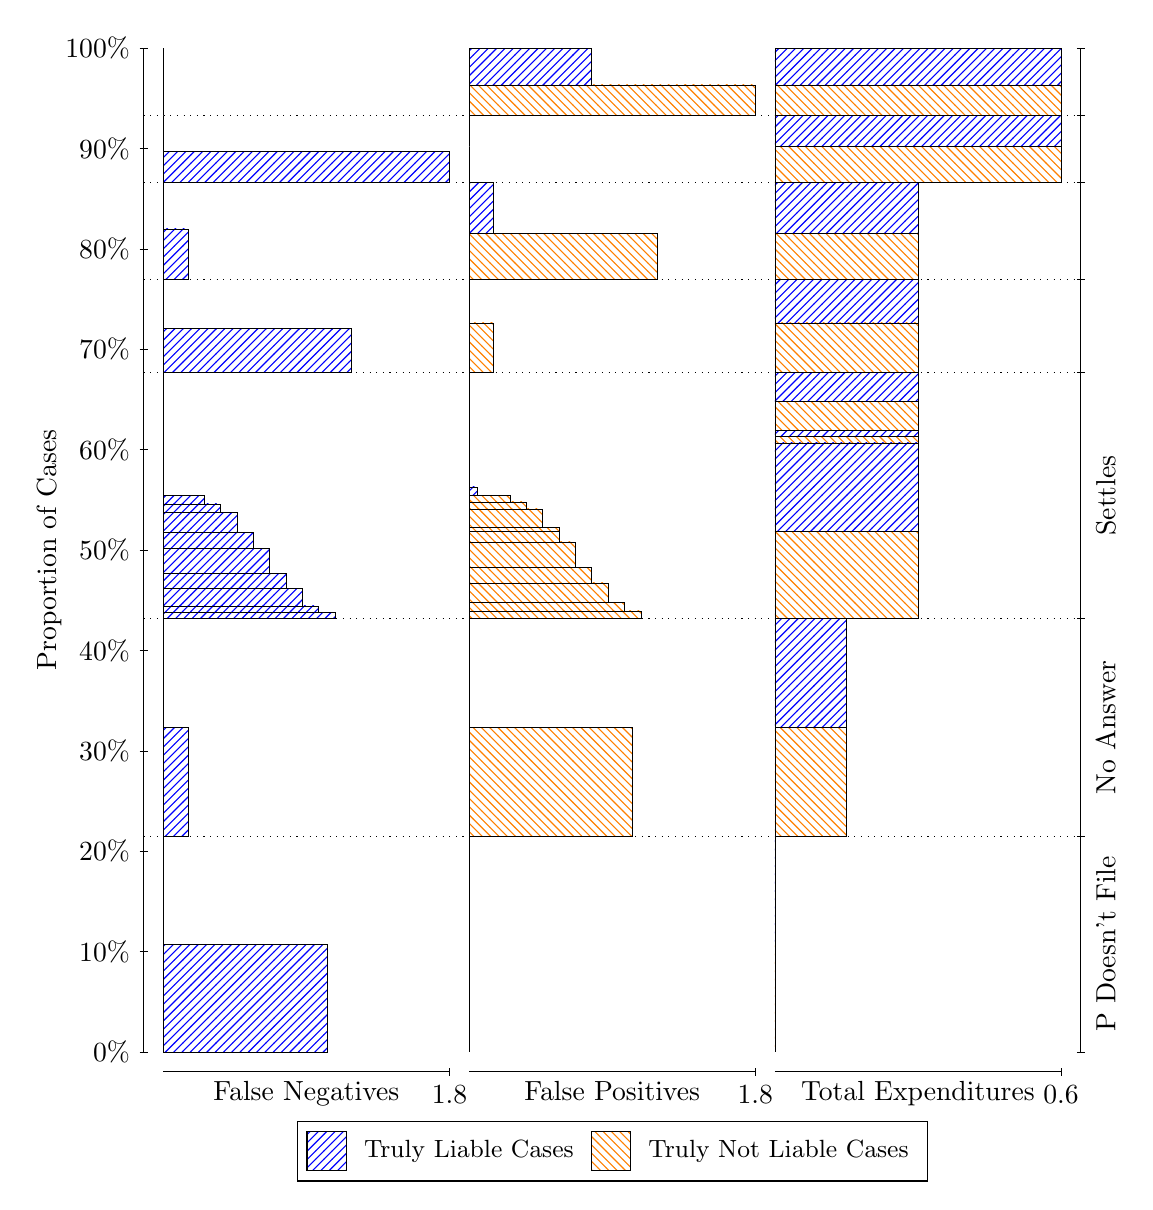
\begin{tikzpicture}
\draw[black, very thin] (1.5,1.75) -- (1.5,14.5);
\node[rotate=90, anchor=center] at (0.3, 8.125) {Proportion of Cases};
\draw[black, very thin] (1.45,1.75) -- (1.55,1.75);
\node[anchor=east] at (1.45, 1.75) {0\%};
\draw[black, very thin] (1.45,3.025) -- (1.55,3.025);
\node[anchor=east] at (1.45, 3.025) {10\%};
\draw[black, very thin] (1.45,4.3) -- (1.55,4.3);
\node[anchor=east] at (1.45, 4.3) {20\%};
\draw[black, very thin] (1.45,5.575) -- (1.55,5.575);
\node[anchor=east] at (1.45, 5.575) {30\%};
\draw[black, very thin] (1.45,6.85) -- (1.55,6.85);
\node[anchor=east] at (1.45, 6.85) {40\%};
\draw[black, very thin] (1.45,8.125) -- (1.55,8.125);
\node[anchor=east] at (1.45, 8.125) {50\%};
\draw[black, very thin] (1.45,9.4) -- (1.55,9.4);
\node[anchor=east] at (1.45, 9.4) {60\%};
\draw[black, very thin] (1.45,10.675) -- (1.55,10.675);
\node[anchor=east] at (1.45, 10.675) {70\%};
\draw[black, very thin] (1.45,11.95) -- (1.55,11.95);
\node[anchor=east] at (1.45, 11.95) {80\%};
\draw[black, very thin] (1.45,13.225) -- (1.55,13.225);
\node[anchor=east] at (1.45, 13.225) {90\%};
\draw[black, very thin] (1.45,14.5) -- (1.55,14.5);
\node[anchor=east] at (1.45, 14.5) {100\%};

\draw[black, very thin] (13.4,1.75) -- (13.4,14.5);
\draw[black, very thin] (13.35,1.75) -- (13.45,1.75);
\node[anchor=west] at (13.35, 1.75) {};
\draw[black, very thin] (13.35,4.4907) -- (13.45,4.4907);
\node[anchor=west] at (13.35, 4.4907) {};
\draw[black, very thin] (13.35,7.2536) -- (13.45,7.2536);
\node[anchor=west] at (13.35, 7.2536) {};
\draw[black, very thin] (13.35,10.382) -- (13.45,10.382);
\node[anchor=west] at (13.35, 10.382) {};
\draw[black, very thin] (13.35,11.561) -- (13.45,11.561);
\node[anchor=west] at (13.35, 11.561) {};
\draw[black, very thin] (13.35,12.789) -- (13.45,12.789);
\node[anchor=west] at (13.35, 12.789) {};
\draw[black, very thin] (13.35,13.643) -- (13.45,13.643);
\node[anchor=west] at (13.35, 13.643) {};
\draw[black, very thin] (13.35,14.5) -- (13.45,14.5);
\node[anchor=west] at (13.35, 14.5) {};

\draw[black, very thin, pattern color=blue, pattern=north east lines] (1.75,1.75) rectangle (3.8262,3.1203);
\draw[black, very thin, pattern color=orange, pattern=north west lines] (1.75,3.1203) rectangle (1.75,4.4907);
\draw[black, very thin, pattern color=blue, pattern=north east lines] (1.75,4.4907) rectangle (2.0614,5.8721);
\draw[black, very thin, pattern color=orange, pattern=north west lines] (1.75,5.8721) rectangle (1.75,7.2536);
\draw[black, very thin, pattern color=blue, pattern=north east lines] (1.75,7.2536) rectangle (3.93,7.3285);
\draw[black, very thin, pattern color=blue, pattern=north east lines] (1.75,7.3285) rectangle (3.7224,7.4149);
\draw[black, very thin, pattern color=blue, pattern=north east lines] (1.75,7.4149) rectangle (3.5148,7.6399);
\draw[black, very thin, pattern color=blue, pattern=north east lines] (1.75,7.6399) rectangle (3.3071,7.8239);
\draw[black, very thin, pattern color=blue, pattern=north east lines] (1.75,7.8239) rectangle (3.0995,8.1458);
\draw[black, very thin, pattern color=blue, pattern=north east lines] (1.75,8.1458) rectangle (2.8919,8.3498);
\draw[black, very thin, pattern color=blue, pattern=north east lines] (1.75,8.3498) rectangle (2.6843,8.6019);
\draw[black, very thin, pattern color=blue, pattern=north east lines] (1.75,8.6019) rectangle (2.4767,8.7095);
\draw[black, very thin, pattern color=blue, pattern=north east lines] (1.75,8.7095) rectangle (2.269,8.8176);
\draw[black, very thin, pattern color=orange, pattern=north west lines] (1.75,8.8176) rectangle (1.75,10.382);
\draw[black, very thin, pattern color=blue, pattern=north east lines] (1.75,10.382) rectangle (4.1376,10.936);
\draw[black, very thin, pattern color=orange, pattern=north west lines] (1.75,10.936) rectangle (1.75,11.561);
\draw[black, very thin, pattern color=blue, pattern=north east lines] (1.75,11.561) rectangle (2.0614,12.204);
\draw[black, very thin, pattern color=orange, pattern=north west lines] (1.75,12.204) rectangle (1.75,12.789);
\draw[black, very thin, pattern color=blue, pattern=north east lines] (1.75,12.789) rectangle (5.3833,13.185);
\draw[black, very thin, pattern color=orange, pattern=north west lines] (1.75,13.185) rectangle (1.75,13.643);
\draw[black, very thin, pattern color=orange, pattern=north west lines] (1.75,13.643) rectangle (1.75,14.033);
\draw[black, very thin, pattern color=blue, pattern=north east lines] (1.75,14.033) rectangle (1.75,14.5);
\draw[black, very thin, pattern color=orange, pattern=north west lines] (5.6333,1.75) rectangle (5.6333,3.1203);
\draw[black, very thin, pattern color=blue, pattern=north east lines] (5.6333,3.1203) rectangle (5.6333,4.4907);
\draw[black, very thin, pattern color=orange, pattern=north west lines] (5.6333,4.4907) rectangle (7.7095,5.8721);
\draw[black, very thin, pattern color=blue, pattern=north east lines] (5.6333,5.8721) rectangle (5.6333,7.2536);
\draw[black, very thin, pattern color=orange, pattern=north west lines] (5.6333,7.2536) rectangle (7.8133,7.3527);
\draw[black, very thin, pattern color=orange, pattern=north west lines] (5.6333,7.3527) rectangle (7.6057,7.4602);
\draw[black, very thin, pattern color=orange, pattern=north west lines] (5.6333,7.4602) rectangle (7.3981,7.7071);
\draw[black, very thin, pattern color=orange, pattern=north west lines] (5.6333,7.7071) rectangle (7.1905,7.9068);
\draw[black, very thin, pattern color=orange, pattern=north west lines] (5.6333,7.9068) rectangle (6.9829,8.2285);
\draw[black, very thin, pattern color=orange, pattern=north west lines] (5.6333,8.2285) rectangle (6.7752,8.3632);
\draw[black, very thin, pattern color=orange, pattern=north west lines] (5.6333,8.3632) rectangle (6.7752,8.417);
\draw[black, very thin, pattern color=orange, pattern=north west lines] (5.6333,8.417) rectangle (6.5676,8.6483);
\draw[black, very thin, pattern color=orange, pattern=north west lines] (5.6333,8.6483) rectangle (6.36,8.7361);
\draw[black, very thin, pattern color=orange, pattern=north west lines] (5.6333,8.7361) rectangle (6.1524,8.8183);
\draw[black, very thin, pattern color=blue, pattern=north east lines] (5.6333,8.8183) rectangle (5.7371,8.9264);
\draw[black, very thin, pattern color=blue, pattern=north east lines] (5.6333,8.9264) rectangle (5.6333,10.382);
\draw[black, very thin, pattern color=orange, pattern=north west lines] (5.6333,10.382) rectangle (5.9448,11.008);
\draw[black, very thin, pattern color=blue, pattern=north east lines] (5.6333,11.008) rectangle (5.6333,11.561);
\draw[black, very thin, pattern color=orange, pattern=north west lines] (5.6333,11.561) rectangle (8.021,12.146);
\draw[black, very thin, pattern color=blue, pattern=north east lines] (5.6333,12.146) rectangle (5.9448,12.789);
\draw[black, very thin, pattern color=orange, pattern=north west lines] (5.6333,12.789) rectangle (5.6333,13.247);
\draw[black, very thin, pattern color=blue, pattern=north east lines] (5.6333,13.247) rectangle (5.6333,13.643);
\draw[black, very thin, pattern color=orange, pattern=north west lines] (5.6333,13.643) rectangle (9.2667,14.033);
\draw[black, very thin, pattern color=blue, pattern=north east lines] (5.6333,14.033) rectangle (7.1905,14.5);
\draw[black, very thin, pattern color=orange, pattern=north west lines] (9.5167,1.75) rectangle (9.5167,3.1203);
\draw[black, very thin, pattern color=blue, pattern=north east lines] (9.5167,3.1203) rectangle (9.5167,4.4907);
\draw[black, very thin, pattern color=orange, pattern=north west lines] (9.5167,4.4907) rectangle (10.425,5.8721);
\draw[black, very thin, pattern color=blue, pattern=north east lines] (9.5167,5.8721) rectangle (10.425,7.2536);
\draw[black, very thin, pattern color=orange, pattern=north west lines] (9.5167,7.2536) rectangle (11.333,8.3632);
\draw[black, very thin, pattern color=blue, pattern=north east lines] (9.5167,8.3632) rectangle (11.333,9.4865);
\draw[black, very thin, pattern color=orange, pattern=north west lines] (9.5167,9.4865) rectangle (11.333,9.5687);
\draw[black, very thin, pattern color=blue, pattern=north east lines] (9.5167,9.5687) rectangle (11.333,9.6436);
\draw[black, very thin, pattern color=orange, pattern=north west lines] (9.5167,9.6436) rectangle (11.333,10.016);
\draw[black, very thin, pattern color=blue, pattern=north east lines] (9.5167,10.016) rectangle (11.333,10.382);
\draw[black, very thin, pattern color=orange, pattern=north west lines] (9.5167,10.382) rectangle (11.333,11.008);
\draw[black, very thin, pattern color=blue, pattern=north east lines] (9.5167,11.008) rectangle (11.333,11.561);
\draw[black, very thin, pattern color=orange, pattern=north west lines] (9.5167,11.561) rectangle (11.333,12.146);
\draw[black, very thin, pattern color=blue, pattern=north east lines] (9.5167,12.146) rectangle (11.333,12.789);
\draw[black, very thin, pattern color=orange, pattern=north west lines] (9.5167,12.789) rectangle (13.15,13.247);
\draw[black, very thin, pattern color=blue, pattern=north east lines] (9.5167,13.247) rectangle (13.15,13.643);
\draw[black, very thin, pattern color=orange, pattern=north west lines] (9.5167,13.643) rectangle (13.15,14.033);
\draw[black, very thin, pattern color=blue, pattern=north east lines] (9.5167,14.033) rectangle (13.15,14.5);
\draw[black, dotted] (1.5,4.4907) -- (13.4,4.4907);
\draw[black, dotted] (1.5,7.2536) -- (13.4,7.2536);
\draw[black, dotted] (1.5,10.382) -- (13.4,10.382);
\draw[black, dotted] (1.5,11.561) -- (13.4,11.561);
\draw[black, dotted] (1.5,12.789) -- (13.4,12.789);
\draw[black, dotted] (1.5,13.643) -- (13.4,13.643);
\draw[black, very thin] (1.75,1.5) -- (5.3833,1.5);
\node[anchor=north] at (3.5667, 1.5) {False Negatives};
\draw[black, very thin] (5.3833,1.45) -- (5.3833,1.55);
\node[anchor=north] at (5.3833, 1.45) {1.8};

\draw[black, very thin] (5.6333,1.5) -- (9.2667,1.5);
\node[anchor=north] at (7.45, 1.5) {False Positives};
\draw[black, very thin] (9.2667,1.45) -- (9.2667,1.55);
\node[anchor=north] at (9.2667, 1.45) {1.8};

\draw[black, very thin] (9.5167,1.5) -- (13.15,1.5);
\node[anchor=north] at (11.333, 1.5) {Total Expenditures};
\draw[black, very thin] (13.15,1.45) -- (13.15,1.55);
\node[anchor=north] at (13.15, 1.45) {0.6};

\node[black, centered, rotate=90] at (13.72, 3.1203) {P Doesn't File};
\node[black, centered, rotate=90] at (13.72, 5.8721) {No Answer};
\node[black, centered, rotate=90] at (13.72, 8.818) {Settles};





\draw (7.449999999999999,1.5) node[draw=none] (baseCoordinate) {};
\begin{scope}[align=center]
        \matrix[scale=0.5, draw=black, below=0.5cm of baseCoordinate, nodes={draw}, column sep=0.1cm]{
            \node[rectangle, draw, minimum width=0.5cm, minimum height=0.5cm, pattern=north east lines, pattern color=blue] {}; &
            \node[draw=none, font=\small] (B) {Truly Liable Cases}; &
            \node[rectangle, draw, minimum width=0.5cm, minimum height=0.5cm, pattern=north west lines, pattern color=orange] {}; &
            \node[draw=none, font=\small] (B) {Truly Not Liable Cases}; \\
            };
\end{scope}

\end{tikzpicture}
\end{document}